\documentclass[two column, twoside, a4paper]{article}

%%% -- Preamble -- %%%
\usepackage[utf8]{inputenc}
\usepackage{dblfloatfix}
\usepackage{float}
\usepackage[polish]{babel}
\usepackage[T1]{fontenc}
\usepackage[backend=biber, maxbibnames=3, style=authoryear, autocite=inline]{biblatex}
\usepackage{fancyhdr}
\usepackage{titlesec}
\usepackage{blindtext}
\usepackage{cuted}
\usepackage[most]{tcolorbox}
\usepackage[columnsep = 1cm,
	    lmargin = 0.6in,
	    rmargin = 0.4in,
	    tmargin = 0.5in,
	    bmargin = 0.65in,
	    headsep = \baselineskip]{geometry}

% Environmental variable for bib file
\addbibresource{$BIB}

% Metadata
\title{Metody biologii molekularnej, w badaniach wirusów}
\author{Jakub J. Guzek}
\date{}

% Section Formatting
\titleformat{\section}
{\sc \bfseries \Large}
{}
{0em}
{}[\titlerule]

\titleformat{\subsection}
{\bfseries \large}
{}
{0em}
{}

\titleformat{\subsubsection}
{\bfseries}
{}
{0em}
{}

% Box formatting
\tcbset{enhanced, colback=orange!15!white, sharp corners, boxrule = 0pt, frame hidden}

% Headers
\pagestyle{fancy}
\fancyhf{}
\fancyhead[RE, LO]{Szkoła Główna Gospodarstwa Wiejskiego}
\fancyhead[LE, RO]{Biotechnologia}
\fancyfoot[LE, RO]{\thepage}
\fancyfoot[RE,LO]{Goździk -- mikrorozmnażanie}
\renewcommand{\footrulewidth}{0.05pt}

%%% -- Body -- %%%
\begin{document}

\begin{strip}
{\sc \bfseries \huge \fontfamily{lmss}\selectfont Goździk -- mikrorozmnażanie} \vspace{\baselineskip}

{\bfseries \large Michał Balcerak, Jakub J. Guzek, Grzegorz Jakubiak, Maria Jóźwiak, Zuzanna Siek, Oliwia Śniadała}

{Szkoła Główna Gospodarstwa Wiejskiego, Biotechnologia}\vspace{\baselineskip}

\hrule
\end{strip}

\section{Wstęp}

Mikrorozmnażanie inaczej mówiąc rozmnażanie klonalne to sposób wegetatywnego rozmnażania roślin w kulturach in vitro tzn. na sztucznych podłożach, przygotowanych przez człowieka w warunkach laboratoryjnych. Najistotniejszym czynnikiem w mikrorozmnażaniu jest skład pożywki. Istotnym jest dokładna zawartość w niej hormonów wspomagających wzrost i rozwój, a także sama struktura wpływająca na przebieg mikrorozmnażania – czy pożywka jest płynna czy stała.

\section{Procedury}

W samej procedurze najczęściej używa się pożywki według \autocite{Murashige1962}\footnote{Pożywka według Murashige’a i Skooga / Pożywka MS – podstawowa pożywka stosowana w kulturach in vitro roślin, tkanek roślinnych i kulturach zawiesinowych komórek roślinnych.} lub jej modyfikację, rzadziej korzysta się z pożywki B5 \autocite{Gamborg1968}

Mikrorozmnażanie możemy podzielić na 3 istotne etapy:
\begin{enumerate}
	\item Założenie kultury
	\item Namnażanie
	\item Ukorzenianie pędów
\end{enumerate}

Najczęstszą techniką mikrorozmnażania stosowaną do rozmnażania klonalnego roślin ozdobnych, w tym goździka jest metoda pędów przybyszowych. Założenie kultury zdaje się być najtrudniejszym etapem ze względu na niebezpieczeństwo zakażenia sterylnych eksplantatów pierwotnych. Eksplantaty te układa się na specjalnie przygotowane pożywki stymulujące wytworzenie pędów przybyszowych lub cebulek. Kolejnym etapem jest namnażanie. Kiedy dojdzie już do wytworzenia pędów przybyszowych, “przesadza się” daną roślinę na pożywkę z dużą zawartością cytokinin odpowiadających za stymulację tworzenia nowych pędów w roślinie, potocznie nazywanych mikrocebulkami. W przypadku goździka, regeneracja pędu przybyszowego odbywa się z międzywęźla i zachodzi z jednoczesnym tworzeniem korzeni.  Goździki najczęściej ukorzenia się in vitro. Stosuje się pożywki z wysoką zawartością auksyn, obniżoną zawartością soli mineralnych, a także dodatkiem węgla aktywnego. Taki skład pożywki usprawnia proces tworzenia korzeni.

\section{Stan produkcji i laboratoria w Polsce}


Goździk (\textit{Dianthus caryophyllus} L.) jest najbardziej znany jako kwiat cięty
z kwiaciarnii, ale  dobrze sprawdza się także jako roślina rabatowa w ogrodzie. Goździk nalezy do rodziny Caryophyllous, która obejmuje  88 rodzajów i 1750 gatunków. Uprawa goździków zaczęła się już ponad 2000 lat temu. Nowoczesne odmiany zostały opracowane po raz pierwszy we Francji w 1840 roku. Nazwa goździk pochodzi od łacińskiego „Carnatio”, co oznacza cielesność, a caryophyllus odnosi się do różowego koloru oryginalnego, kwitnącego gatunku. Jest to roślina wieloletnia, lubiąca stanowiska nasłoniecznione I powietrze wypełnione solą. Nie lubi kwaśnej gleby, ale toleruje zakres pH od 6-8. Gożdzik to roślina, która ma opinię jednego z najważniejszych na świecie kwiatów ciętych z powodu ciągłego kwitnienia  oraz odmian jedno- i wielokolorowych.
Kwiat goździka jest wspaniałym akcentem dla bukietów, ale ma swoje zastosowanie  jako niekonwencjonalna roślina spożywcza. Jest stosowany w sałatkach ozdoby,
w sałatkach owocowych i do aromatyzowania owoców itp. Może być stosowany jako substytut płatków róży w produkcji syropu. Olejek eteryczny pozyskiwany  z kwiatów, wykorzystywany jest powszechnie w perfumerii (500kg kwiatów wytwarza 100g oleju) .

\begin{figure}[tp]
	\begin{tcolorbox}
		\centering
		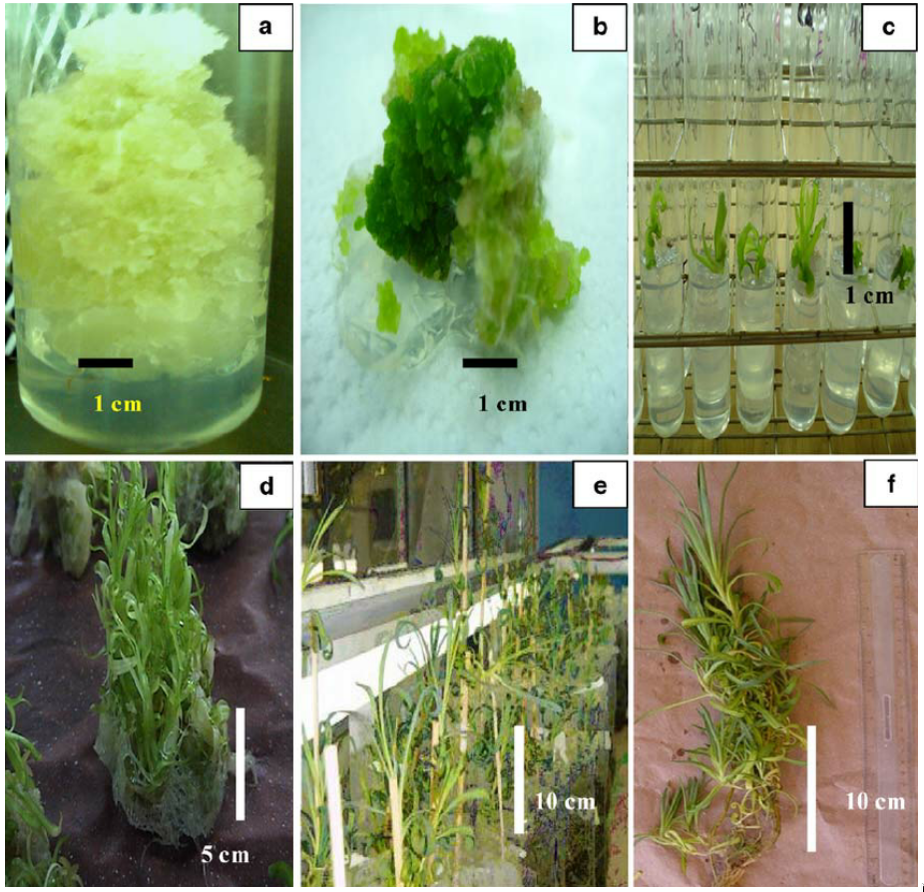
\includegraphics[width=\textwidth]{./figure1.png}
		\caption{Mikrorozmnażanie \textit{Dianthus caryophyllus}. (a) Kallus na pożywce wzrostowej dla kallusa (\textit{ang. callus growth medium}). (b) Kallus embriogenny. (c) proliferacja łodyżki (d) ukorzeniające się rośliny. (e) rośliny \textit{ex vitro} po 12 tygodniach. (f) rośliny po 28 tygodniach. Na Podstawie (Gutiérrez-Miceli, Arias 2010)}
	\end{tcolorbox}
\end{figure}

W Polsce obecnie działa około 40 laboratoriów zajmujących się mikrorozmnażaniem. Głównie dotyczy to roślin ozdobnych takich jak: gerbera, różanecznik, azalia, storczyk, fikus, lilia, chryzantema, gloksynia, goździk, paproć, primula, a także borówki wysokiej, truskawki, żurawiny i jeżyny. Polskie sadzonki są eksportowane w większości do Holandii, Anglii, Izraela, Węgier, Czech, Białorusi, Bułgarii, Turcji, USA oraz na Ukrainę, Litwę i Łotwę. Krajowa produkcja wypełnia potrzeby rynkowe, rocznie produkuje się in vitro ok. 70-100 mln sadzonek. Jest to jedna z największych produkcji sadzonek in vitro w Europie. Szacuje się, że na świecie produkuje się ok. 800 mln sadzonek rocznie obejmujących łącznie 300 gatunków, głównie roślin ozdobnych. Natomiast jeśli chodzi o produkcję europejską to szacuje ona na ok. 200 mln sadzonek rocznie. Głównym producentem jest Holandia, kolejno: Francja, Polska, Włochy i Niemcy.

Pomimo częstego zjawiska witryfikacji, niektóre gatunki goździka (\textit{Dianthus}) poddaje się mikrorozmnażaniu. Eksplantaty mogą pochodzić z różnych części rośliny, jednak w przypadku mikrorozmnażania komercyjnego goździka ogorodowego (\textit{D. caryophyllus}) najczęściej stosuje się wierzchołki pędów, z których regenerowana jest roślina. Opisano również mikrorozmnażanie tego gatunku z wykorzystaniem: fragmentów łodygim liści, pąków bocznych, węzłów, zalążków i płatków korony. Pomyślnie przebiega również mikrorozmnażanie goździka chińskiego (\textit{D. chinensis}) z wykorzystaniem fragmentów liści, goździka pysznego (\textit{D. superbus}) z wykorzystaniem protoplastów mezofilu oraz dwóch kultywarów goździka sinego (\textit{D. grationopolitanus}). Mikrorozmnażanie stwarza perspektywy skutecznego rozmnażania roslin zagrożonych wyginięciem. Prowadzono badania nad mikrorozmnażaniem \textit{Dianthus petraeus ssp. simonkaianus.} oraz \textit{Dianthuspyrenaicus Pourr} \autocite{Fraga2004}.


\section{Udział produkcji \textit{in vitro} w produkcji ogólnej}

Rozmnażanie klonalne ma ogromne znaczenie ekonomiczne. Podstawową zaletą procedury jest uzyskanie ogromnej ilości roślin z małej ilości pierowtnych eksplantatów w bardzo krótkim czasie. Oczywiście wydajność procesu zależy od odmiany, rodzaju eksplantatu, doboru i składu pożywki, warunków fizycznych kultury oraz przeprowadzanych subkultur. Mikrorozmnażanie pozwala również zaoszczędzić powierzchnię, w której normalnie prowadzilibyśmy uprawę danej odmiany. Stosowanie tej techniki przynosi również pewne zalety dotyczące przechowywania roślin oraz ich transportu. Aby zachować roślinę w pełni sił witalnych, stosuje się technikę przechowywania zregenerowanych roślinek przez kilka miesięcy w obniżonej temperaturze.
Produkcja roślin przez mikrorozmnażanie jest niezależna od czynników klimatycznych, co ogólnie wpływa na brak strat spowodowanych kataklizmami takimi jak susza.

\section{Znaczenie ekonomiczne}

Wysuszone główki kwiatowe są również stosowane w kosmetykach. Mówi się, że kwiaty goździka wykazują działanie przeciwskurczowe, kardiotoniczne, ale również napotne i wywołujące napięcie nerwowe (Chopra i in., 1986).
W ciągu ostatnich 40 lat, zapotrzebowanie rynkowe na goździki znacznie wzrosło. Przyglądając się liczbom możemy zaobserwować ogromny wzrost zainteresowania tą rośliną ozdboną. Zużycie goździków na światowym rynku kwiatowym w 1985 r. szacowało na  około 12,5 miliardów dolarów. W 1990 r. całkowita konsumpcja wzrosła do około 25 miliardów dolarów. W 1995, całkowite zużycie wzrosło do 31 miliardów dolarów. Ciągły rozwój w technoogii produkcyjnych, importu i zmiennych ekonomicznych spowodowało wzrost zapotrzebowania goździka na rynku światowym, do 35 miliardów dolarów w 2000 roku.
Głównymi światowymi eksporterami goździków są Europa, Ameryka Łacińska i Izrael.
Ameryka łacińska eksportuje goździki na rynek europejski i amerykański, np. Meksyk, Kostarykę, Kolumbię, Peru, Chile, Argentynę i Dominikanę. Kraje azjatyckie, takie jak Japonia, Indie i Pakistan koncentrują się również na produkcji goździków. Wobec
zalety tych upraw i zaspokojenie światowego zapotrzebowania na goździki, kraje te zaczęły stosować technikę rozmnażania wegetatywnego.

\section{Podsumowanie}

Mikrorozmnazanie jest metodą, która z roku na rok cieszy się coraz większym zainteresowaniem wśród firm zajmujących się sadzonkami. Wszelkie metody obejmujące wykorzystanie romnazania klonalnego są stale udoskonalane w celu zwiększenia wydajności, zniwelowania trudności związanych z przebiegiem procesu, a także w celu obniżenia kosztów produkcyjnych. Szacuje się, że za 15 lat proces ten będzie odgrywał najistotniejszą rolę w produkcji roślin ozdobnych i nie tylko. Goździk jest wyłącznie jedną z wielu rodzajów roślin, na które wzrósł popyt w ciągu ostatnich 20lat. Przypuszcza się również że ze względu na zmieniający się klimat i nieodwracalne zmiany zachodzące w środowisku naturalnym, mikrorozmnazanie będzie jedynym rozwiązaniem pozwalającym na uprawę i rozmnażanie roślin.

\nocite{Malepszy2004, Mulcahy1975, Jain1997, Gutierrez2010, Fraga2004, Forkmann1980, Casas2009, Ahmadian2017}
\printbibliography

\end{document}
